% Context-guided unified four-task forecasting study for IEEE Transactions on Smart Grid.
\documentclass[journal]{IEEEtran}
\usepackage[T1]{fontenc}
\usepackage{cite}
\usepackage[hyphens]{url}
\usepackage{graphicx}
\usepackage{xcolor}
\usepackage{booktabs}
\usepackage{needspace}
\usepackage{array}
\usepackage{multirow}
\usepackage{amsmath}
\usepackage{amssymb}
\usepackage{algorithm}
\usepackage{algpseudocode}
\usepackage[hidelinks]{hyperref}
\usepackage{placeins}
\AddToHook{cmd/bibliography/before}{\FloatBarrier}
\urlstyle{rm}
\newcolumntype{L}[1]{>{\raggedright\arraybackslash}p{#1}}
\newcommand{\metricstd}[1]{\kern.20em\makebox[2.30em][l]{#1}}
\newcommand{\bestmetric}[2]{{\bfseries #1$\kern.20em\boldsymbol{\pm}$\kern.20em\makebox[2.30em][l]{#2}}}
\newcommand{\secondmetric}[2]{\underline{#1$\kern.20em\pm$\kern.20em\makebox[2.30em][l]{#2}}}
\setcounter{topnumber}{3}
\setcounter{dbltopnumber}{3}
\setcounter{totalnumber}{4}
\renewcommand{\topfraction}{0.95}
\renewcommand{\dbltopfraction}{0.95}
\renewcommand{\textfraction}{0.05}
\renewcommand{\floatpagefraction}{0.8}
\renewcommand{\dblfloatpagefraction}{0.8}
\setlength{\floatsep}{12pt plus 2pt minus 2pt}
\setlength{\dblfloatsep}{12pt plus 2pt minus 2pt}
\setlength{\textfloatsep}{12pt plus 2pt minus 2pt}
\setlength{\dbltextfloatsep}{12pt plus 2pt minus 2pt}
\makeatletter
\setlength{\@fptop}{0pt}
\setlength{\@fpsep}{12pt}
\setlength{\@fpbot}{0pt plus 1fil}
\setlength{\@dblfptop}{0pt}
\setlength{\@dblfpsep}{12pt}
\setlength{\@dblfpbot}{0pt plus 1fil}
\makeatother
\title{EnergyCA-LLM: Context-Guided Window-Adaptive Residual Learning for Unified Renewable Generation and Load Forecasting}
\author{Kai Yang,~\IEEEmembership{Student Member,~IEEE,}
        Jianian Hua,~\IEEEmembership{Student Member,~IEEE,}
        Tianxiang Cui,~\IEEEmembership{Senior Member,~IEEE,} \\
        Heng Yu,~\IEEEmembership{Senior Member,~IEEE,}
        Goran Strbac,~\IEEEmembership{Fellow,~IEEE,}
        and Yujian Ye,~\IEEEmembership{Senior Member,~IEEE}
% \vspace{-1.0em}     
% \thanks{This work has been supported in part by the National Natural Science Foundation of China under Grant 52207082, in part by the Natural Science Foundation of Jiangsu Province under Grant BK20220842 and in part by CCF-Tencent Rhino-Bird Open Research Fund under Grant CCF-Tencent RAGR20230110. \textit{(Corresponding Author: Yujian Ye)}.}
% \thanks{Jianxiong Hu and Yujian Ye are with the School of Electrical Engineering, Southeast University, Nanjing 210096, China (e-mail: cuihan@seu.edu.cn). }
% \thanks{Yujian Ye is with the School of Electrical Engineering and Jiangsu Provincial Key Laboratory of Smart Grid Technology and Equipment, Southeast University, Nanjing 210096, China (e-mail: yeyujian@seu.edu.cn). }
}




\begin{document}
\raggedbottom
\bstctlcite{TSGReferenceStyle}
\maketitle

\begin{abstract}
Electricity demand, wind power, photovoltaic generation and net load share temporal structure but differ in physical drivers and forecast-time information. EnergyCA-LLM unifies these tasks in a shared numerical predictor with layerwise semantic--numerical residual control: frozen language representations, numerical history and context-group availability determine window-specific coefficients over low-rank correction bases after each temporal block. A shared decoder and task-balanced objective retain native task interfaces, while source-trained bases and target-window coefficient synthesis support zero-shot deployment through the same controller. Three-seed gate and availability studies across four energy benchmarks, complemented by reference comparisons of parameter sharing and context encoders, examine contextual control under different information conditions. A field-level language study on CAISO records four-target mean MASE reductions of 16.40\% and 9.63\% with 30 and 90 training days.
\end{abstract}

\begin{IEEEkeywords}
Energy forecasting, large language models, load forecasting, photovoltaic power forecasting, residual adaptation, unified forecasting, wind power forecasting.
\end{IEEEkeywords}

\section{Introduction}
\label{sec:introduction}

\IEEEPARstart{T}{he} integration of wind and photovoltaic (PV) generation makes electricity demand, renewable production and net-load forecasting central to power-system scheduling and balancing. Forecasts inform reserve allocation and renewable integration, while smart-meter measurements broaden the data available for demand analysis~\cite{wang2019smartmeterreview,browell2021regionalNetLoad,devilmarest2024adaptive}. These targets share calendar, weather and temporal influences but respond differently: demand reflects activity and temperature, wind power depends on atmospheric and turbine conditions, and PV output follows irradiance and plant characteristics. Net load describes the remaining demand according to its regional source definition. Sharing forecasting parameters across these targets requires preserving their distinct operational meanings.

Energy-specific predictors capture this heterogeneity in several ways. Recurrent load models and baseline-refinement profiles represent demand variability~\cite{kong2019residentiallstm,xiao2024baselinerefine}, while transfer regression and graph-based transfer learning exploit related households~\cite{wu2020transferload,wu2023gnntransfer}. Wind forecasting combines feature-based multi-step prediction with adaptive probabilistic learning~\cite{decaro2022dafte,meng2024metawind}. Multi-site PV prediction uses spatial dependencies, and multimodal approaches select irradiance inputs or combine satellite imagery with production series~\cite{simeunovic2022graphpv,jing2025solarfusionnet,wang2025robustmultimodalpv}. Regional net-load predictors include conditional-extreme, adaptive and computationally simple MLP models~\cite{browell2021regionalNetLoad,devilmarest2024adaptive,faustine2025efficiency}. These studies establish strong task-specific references; a unified predictor must additionally determine how their different contexts should modify shared temporal features.

Parameter sharing has precedents in pooled household prediction and multi-task electricity demand forecasting~\cite{shi2018poolingrnn,fiot2018multitask}, as well as coupled multi-energy models for electricity, heating and cooling loads using BiLSTM and Bayesian Transformers~\cite{guo2022bilstmmultienergy,wang2024bayesianmultienergy}. Here, the Load, Wind, PV and Net-load datasets are independently sourced, and one jointly trained predictor serves their native cadences and horizons. Sharing temporal structure across these task families therefore requires contextual control that responds to the task, recent trajectory and available information.

This contextual control must use information available at each forecast origin. Data cleansing and imputation address incomplete load measurements~\cite{mateos2013lowrank}, and available-feature-adaptive energy forecasters accommodate missing inputs~\cite{stratigakos2026missingadaptive}. Forecasting also distinguishes valid time from release time: an issued weather forecast and a later realization may describe the same future interval, but only an eligible release can enter the prediction. The same boundary governs numerical covariates and their textual descriptions, allowing the predictor to condition corrections on eligible context and its age.

Task descriptions and operating states give numerical trajectories their meaning across energy tasks, while pretrained language models offer reusable representations of these descriptions. This motivates a common semantic interface for unified forecasting. Related applications include BERT-based wind prediction in Wind2vec-BERT and explanation-enhanced federated LLM fine-tuning for PV forecasting~\cite{yu2025windbert,song2026llmpv}; general forecasting studies also explore language-model reprogramming and the contribution of pretrained representations~\cite{jin2024timellm,tan2024llmts_critique}.

Conditional adaptation connects such context to numerical feature correction. LoRA supplies low-rank updates~\cite{hu2022lora}; HyperLoRA generates adapters from task descriptions~\cite{lv2024hyperlora}, and C-LoRA adapts time-series channels~\cite{nie2024clora}. LoRA-Flow dynamically combines trained adapters during generation~\cite{wang2024loraflow}, CCM-LoRA routes rank directions under a compute budget~\cite{rafiuddin2026ccmlora}, and LoGo selects adapters per instance~\cite{lee2026logo}. For energy forecasting, windows in the same semantic category can still have different recent trends and information conditions. We therefore construct a joint state from semantics, continuous numerical history and forecast-origin availability to control the shared predictor.

EnergyCA-LLM forms this state through parallel concatenation and semantic--numerical interaction branches, then uses layer-specific heads to generate coefficients over shared low-rank bases. The bases learn reusable correction directions across tasks, while the coefficients combine them for each window after each temporal block. A frozen language encoder, shared numerical predictor and common decoder preserve native task interfaces under a task-balanced objective; zero-shot cross-dataset deployment reuses the source-trained bases and generates target-window coefficients through the same controller. The contributions are as follows:
\begin{itemize}
\item A forecast-origin-aware formulation of unified Load, Wind, PV and Net-load prediction that retains native task interfaces and derives numerical and semantic inputs from the same admissible information set.
\item A joint-state residual controller that combines semantic context, numerical history and availability through concatenation and explicit semantic--numerical interaction, then generates layer-specific coefficients over shared low-rank bases to synthesize window-specific correction operators for zero-shot cross-dataset deployment.
\item Three-seed gate and availability studies of EnergyCA-LLM across four energy tasks, complemented by reference comparisons of parameter sharing and context encoders and field-level studies of language adaptation and CAISO training-label budgets.
\end{itemize}

\section{Problem Formulation}
\label{sec:problem}

Let $\mathcal Q=\{\mathrm{Load},\mathrm{Wind},\mathrm{PV},\mathrm{Net\ load}\}$ denote four task families represented by independent datasets, each retaining its source target definition and units, including the supplied regional net-load series. A forecast window $\omega_i=(q_i,a_i,t_i,L_i,H_i)$ specifies task $q_i$, asset or region $a_i$, issuance time $t_i$, $L_i$ historical steps and $H_i$ target steps, with scalar target sequence $\mathbf y_i\in\mathbb R^{H_i\times1}$.

The admissible information set $\mathcal I_{i,t_i}^{\mathrm{avail}}$ contains static attributes $\mathbf u_i$, historical targets $\mathbf x_i$ and covariates $\mathbf z_i^{\mathrm{hist}}$ available by the observation cutoff, and future-valid inputs $\mathbf z_i^{\mathrm{known}}$ available at issuance. Both numerical inputs and serialized context $s_i$ derive from this set. A channel mask $\mathbf M_i$ accompanies historical values, while a context-group availability vector $\mathbf m_i$ enters the semantic controller; their granularities are specified in the method.

One shared predictor $F_{\Theta;\Phi}$ produces forecasts $\hat{\mathbf y}_i$ through the task interface $(q_i,\Delta_i,\boldsymbol\ell_i)$, where $\Delta_i$ is the sampling interval in minutes and $\boldsymbol\ell_i$ maps output indices to leads in hours, giving valid time $t_i+\ell_{i,h}$. Task and cadence embeddings condition the shared predictor. Training freezes pretrained language weights $\Phi$ and learns $\Theta$, comprising the numerical predictor, semantic projection, controller and residual adapters; numerical transformations, context thresholds and reference scales are fitted on source training partitions. Window adaptation changes control coefficients with the input while fitted parameters remain fixed during prediction.

Zero-shot cross-dataset forecasting applies the source-trained, source-selected EnergyCA-LLM checkpoint to an unseen dataset within $\mathcal Q$. A fixed interface maps target fields and units to source channels and retains the trained task, cadence and forecast-lead schedule. Target histories, static descriptions and eligible calendar inputs condition the forward pass, with model weights, numerical transformations and descriptor thresholds fixed at their source-derived values and checkpoint selection based on source validation data.

\section{EnergyCA-LLM Forecasting Method}
\label{sec:method}

\begin{figure*}[!t]
\centering
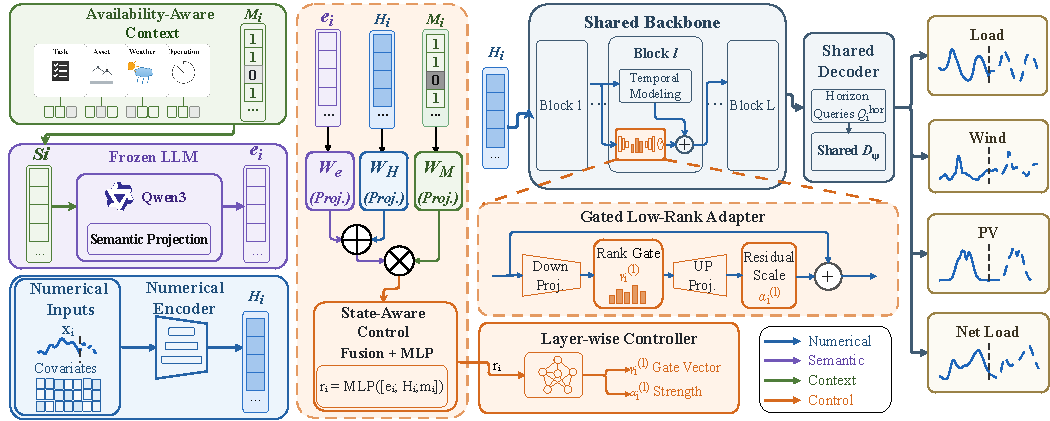
\includegraphics[width=\textwidth]{Figures/energyca_llm_framework.pdf}
\caption{EnergyCA-LLM with layerwise window-conditioned residual control. Available context and numerical histories produce complementary states that control the component weights and strength of layer-specific low-rank residual adapters. Shared weights serve all four tasks at their native cadences. The inset details the adapter computation. Green mask symbols represent context-group availability; the semantic projection is trainable while language-encoder weights are frozen. Blue, purple, green and orange arrows denote numerical, semantic, context and control flows, respectively.}
\label{fig:framework}
\end{figure*}

Figure~\ref{fig:framework} summarizes EnergyCA-LLM. A frozen Qwen3-8B encoder provides one semantic vector per forecast window. The controller combines this vector with numerical history and context-group availability to generate coefficients for the low-rank residual adapter after each of four temporal blocks. The shared horizon-query decoder maps the adapted features to native-horizon forecasts.

% \subsection{Forecast-Origin Encoding}
\subsection{Semantic Representation}

% \paragraph{Eligible fields and missingness.}
% For a candidate field $f$ with valid time $\tau$, let $\rho_f(\tau)$ denote its recorded release or observation-arrival time. An eligibility indicator is
% \begin{equation}
% \label{eq:field-eligibility}
% b_{i,f,\tau}=\mathbb I\{\rho_f(\tau)\leq t_i\}\,
% \mathbb I\{\text{field value is available}\}.
% \end{equation}
% Static attributes and calendar variables can be available before their valid time. Equation~\eqref{eq:field-eligibility} determines field inclusion from availability at issuance. The experimental numerical inputs comprise historical observations and known-future calendar variables.
%
% The numerical mask $\mathbf M_i$ accompanies each historical step and channel. It records channel presence and the prescribed removal and delay conditions. A separate field vector $\mathbf m_i\in\{0,1\}^{F}$ describes the context groups available to the controller. After training-only normalization, unavailable numerical entries are set to zero and accompanied by $\mathbf M_i$, distinguishing them from observed zeros. Removing explicit availability encoding leaves numerical masks, observation-age fields and current/older source labels intact; the comparison isolates the additional vector and availability text block.
%
% \paragraph{Deterministic context construction.}
% The constructor $s_i=\mathcal C(\mathcal I_{i,t_i}^{\mathrm{avail}},\mathbf m_i,q_i,a_i)$ uses a fixed order for task, asset, available geographic attributes, issuance time, calendar, weather, recent operation and availability. Source tags distinguish static attributes, observed values, issued forecasts and known-future variables. Only available fields contribute value-bearing text. Continuous observations remain numerical; text carries low-cardinality operating descriptors. Training-history terciles define level, trend and identified weather regimes. Delayed descriptions use observations at the prescribed cutoff and explicitly encode their age.
%
The deterministic string $s_i$ records task, asset, cadence, horizon, issuance hour/month, known calendar, operating descriptors and observation age in a fixed order. Operation level is the latest available daily mean, trend is the difference between the means of the latest three and preceding three observations, and identified weather channels use daily means. Training-history terciles convert these statistics into three relative categories while continuous trajectories remain numerical inputs. The accompanying vector $\mathbf m_i\in\{0,1\}^{10}$ records task, asset, geography, calendar, capacity, current weather, current operation, older weather, older operation and observation age.



We use frozen Qwen3-8B~\cite{qwen2025technicalreport} with $d_{\mathrm{LLM}}=4096$ and descriptions limited to 512 tokens. For $T_i^{\mathrm{text}}$ tokens, its final states are $\mathbf Z_i^{\mathrm{LLM}}\in\mathbb R^{T_i^{\mathrm{text}}\times d_{\mathrm{LLM}}}$. Masked mean pooling followed by a trainable projection gives
\begin{equation}
\label{eq:semantic-representation}
\begin{aligned}
\mathbf z_i^{\mathrm{sem}}
&=\frac{\sum_{j=1}^{T_i^{\mathrm{text}}}\eta_{i,j}\mathbf Z_{i,j}^{\mathrm{LLM}}}
{\sum_{j=1}^{T_i^{\mathrm{text}}}\eta_{i,j}},\\
\mathbf e_i&=\operatorname{LN}(\mathbf W_e\mathbf z_i^{\mathrm{sem}})
\in\mathbb R^d.
\end{aligned}
\end{equation}
Here $\eta_{i,j}$ is one for nonpadding tokens and zero otherwise, and $d=128$. The frozen pooled vector is reused while the projection and layer normalization learn jointly with the predictor.
% Complete serialized strings are encoded with a maximum length of 512 tokens. Frozen vectors can be cached by their complete serialized text and reused across seeds and repeated windows. Changes in field availability, descriptors or observation age require the corresponding context vector.


% \paragraph{Window-level construction.}
% The ten availability entries describe task, asset, geography, calendar, capacity, current weather, current operation, older weather, older operation and observation age. Current and older descriptors identify the observation interval used by the constructor. For example, a delayed weather field contributes its older regime and age together with the corresponding availability entries. A removal condition instead changes the numerical channel mask and the set of serialized descriptors. The same condition is applied before numerical embedding and semantic encoding.
%
% For recent operation, the level descriptor uses the mean over the latest available daily cycle. The trend descriptor uses the difference between the means of the latest three observations and the preceding three observations. Training-window terciles map these statistics to three categorical levels. Weather descriptors apply the same tercile construction to the daily mean of identified weather channels. Task and asset identifiers, native cadence, forecast horizon and issuance information provide the remaining context. Once fitted, these transformations produce a deterministic string for each information set.
%
% Caching is keyed by this complete string. Consequently, two windows with identical context share the frozen pooled vector, while their numerical stem states remain window specific. The trainable projection maps the language vector to the backbone width, and the controller combines it with the trajectory summary and availability vector. This arrangement connects reusable semantic descriptions to continuously varying numerical observations.
%
\subsection{Shared Numerical Backbone and Decoder}

% Each task's historical target, calendar channels and observed covariates form a normalized matrix $\mathbf X_i\in\mathbb R^{L_i\times C}$. Channels retain a fixed input order and are padded to the common width $C=30$. Concatenating values and masks along channels, a length-$P$ patch with stride $S$ is mapped to a temporal token:
The history $\mathbf X_i\in\mathbb R^{L_i\times C}$ has $C=30$ slots: the target, four calendar channels and up to 25 task-specific historical covariates. Unused slots are zero. Its mask $\mathbf M_i\in\{0,1\}^{L_i\times C}$ marks source-channel presence and prescribed removal/delay cutoffs. Zeroed unavailable slots carry mask zero; observed zeros carry mask one. The shared projection therefore consumes a fixed channel layout conditioned by task identity. We flatten each length-$P$ patch at stride $S$ as $\mathbf p_{i,n}=\operatorname{vec}([\mathbf X_i,\mathbf M_i]_{nS:nS+P-1})$ and form its temporal token by
\begin{equation}
\label{eq:numerical-representation}
\mathbf H_{i,n}^{(0)}=\operatorname{Stem}(\mathbf W_p\mathbf p_{i,n})
+\mathbf E_n^{\mathrm{pos}}+\mathbf e_{q_i}^{\mathrm{task}}
+\mathbf e_{\Delta_i}^{\mathrm{cad}}.
\end{equation}
Here $P=16$, $S=8$, $N_i=1+\lfloor(L_i-P)/S\rfloor$ and $n=0,\ldots,N_i-1$. A layer-normalized linear stem maps each $2CP=960$-dimensional patch to $d=128$, with position, task and cadence embeddings identifying its token index, task family and registered 60-, 10- or 30-minute interval. In parallel, four known-future calendar values and the ten entries of $\mathbf m_i$ pass through a shared $14$-to-$128$ projection and position/task/cadence embeddings to form $\mathbf T_{i,\mathrm{known}}\in\mathbb R^{H_i\times128}$. Historical covariates remain in $\mathbf X_i$; this auxiliary sequence carries calendar information and availability.
% The hourly Load history produces 20 tokens, while the 10-minute Wind history produces 125.

% The auxiliary sequence $\mathbf T_{i,\mathrm{known}}$ embeds future known covariates and field availability. In the gate and availability experiments it contains four calendar channels and the ten-dimensional field vector $\mathbf m_i$, together with positional, task and cadence embeddings. Static attributes enter through the context description, and historical weather and SCADA variables enter the historical numerical stream.


Starting from $\mathbf G_i^{(0)}=\mathbf H_i^{(0)}$, each temporal block performs three pre-normalized residual operations:
\begin{equation}
\label{eq:temporal-block}
\begin{aligned}
\mathbf U_i^{(l)}&=\mathbf G_i^{(l-1)}
+\mathcal D\!\left(\operatorname{SA}_l
(\operatorname{LN}_{l,s}(\mathbf G_i^{(l-1)}))\right),\\
\mathbf V_i^{(l)}&=\mathbf U_i^{(l)}
+\mathcal D\!\left(\operatorname{CA}_l
(\operatorname{LN}_{l,c}(\mathbf U_i^{(l)}),\mathbf T_{i,\mathrm{known}})\right),\\
\mathbf H_i^{(l)}&=\mathbf V_i^{(l)}
+\mathcal D\!\left(\operatorname{FFN}_l
(\operatorname{LN}_{l,f}(\mathbf V_i^{(l)}))\right).
\end{aligned}
\end{equation}
Here $\operatorname{SA}_l(\mathbf X)$ is multi-head attention with queries, keys and values from $\mathbf X$, whereas $\operatorname{CA}_l(\mathbf X,\mathbf T)$ uses queries from $\mathbf X$ and keys and values from $\mathbf T$. Thus, known-future tokens condition the historical features before residual adaptation. The FFN has widths $d\!\rightarrow\!4d\!\rightarrow\!d$, a GELU activation and internal dropout; $\mathcal D$ denotes output dropout, omitted at inference. The $K=4$ blocks use four heads, FFN width $4d=512$ and dropout $0.1$. Each block's adapter maps $\mathbf H_i^{(l)}$ to $\mathbf G_i^{(l)}$ for the next layer. Blocks, bases and gates differ across layers, while all tasks and windows share these parameters, the decoder and output head.

For $h=1,\ldots,H_i$, the decoder uses indexed horizon queries $\mathbf Q_{i,h}=\mathbf E_{h-1}^{\mathrm{pos}}+\mathbf e_{q_i}^{\mathrm{task}}+\mathbf e_{\Delta_i}^{\mathrm{cad}}$ and produces
\begin{equation}
\label{eq:shared-decoder}
\mathbf p_i^{\mathrm{out}}=\operatorname{Out}\!\left(
\mathbf Q_i+\operatorname{CrossAttn}(\mathbf Q_i,
\mathbf G_i^{(K)},\mathbf G_i^{(K)})\right).
\end{equation}
The shared decoder restores the $H_i\times1$ forecast as $\hat{\mathbf y}_i=\nu_i\mathbf p_i^{\mathrm{out}}+\mu_i$ using source-fitted scale $\nu_i$ and offset $\mu_i$. Its output indices are associated with valid times through $\boldsymbol\ell_i$, and the fixed source-channel interface represents omitted covariates by zero values and zero masks.


% \paragraph{Task interfaces and tensor dimensions.}
% A batch contains windows from one task and uses that task's native history and horizon lengths. Four such batches contribute to each optimizer update. This organization retains a shared channel layout and shared weights while giving each attention operation a task-specific sequence length. The historical patch contains $2CP=960$ entries from the values and their channel masks, and $\mathbf W_p$ maps this vector to dimension 128. The known-future input has $4+10=14$ entries per horizon position before its auxiliary projection.
%
% Across the four tasks, $\mathbf H_i^{(l)}$ has shape $N_i\times128$, the known sequence and decoder queries have shape $H_i\times128$, and the adapter intermediate has shape $N_i\times8$. The component weights broadcast over temporal tokens, applying one window-level correction operator at every token in a layer. Layer-specific bases and gate projections supply different operators across depth. The shared output head maps each horizon state to one target value, and the training-fitted target transformation restores its processed physical units.
%
% The valid-time mapping associates decoder position $h$ with the physical forecast lead supplied by the task interface. Load and PV have hourly positions, Wind has 10-minute positions, and Net load has half-hour positions. The task and cadence embeddings tell the shared network how to interpret those native indices, while the decoder query count specifies the output horizon.
%
\subsection{Semantic--Numerical Residual Control}

The controller combines coarse semantic descriptions, continuous trajectories and current information conditions into one window state. A learned query $\mathbf w_p\in\mathbb R^d$ pools the stem tokens into a trajectory summary:
\begin{equation}
\label{eq:joint-state-input}
\begin{aligned}
\boldsymbol\pi_i&=\operatorname{softmax}
\!\left(\frac{\mathbf H_i^{(0)}\mathbf w_p}{\sqrt d}\right),\\
\bar{\mathbf H}_i&=\sum_{n=0}^{N_i-1}\pi_{i,n}\mathbf H_{i,n}^{(0)}.
\end{aligned}
\end{equation}
The attention weights sum to one over the historical tokens. We project context-group availability as $\mathbf v_i=\mathbf W_m\mathbf m_i\in\mathbb R^d$ and concatenate the three states into $\mathbf c_i=[\mathbf e_i;\bar{\mathbf H}_i;\mathbf v_i]\in\mathbb R^{3d}$. The joint control state is then
\begin{equation}
\label{eq:window-residual-code}
\begin{aligned}
\mathbf h_i^{\mathrm{ctrl}}&=\operatorname{SiLU}(\mathbf W_1\mathbf c_i),\\
\mathbf b_i&=(\mathbf W_2\mathbf e_i)\odot(\mathbf W_3\bar{\mathbf H}_i),\\
\mathbf r_i&=\operatorname{LN}(\mathbf W_4[\mathbf h_i^{\mathrm{ctrl}};\mathbf b_i])
\in\mathbb R^{d}.
\end{aligned}
\end{equation}
The concatenation branch retains the individual semantic, numerical and availability states, while the product branch explicitly captures coordinate-wise interactions between projected semantics and numerical features. This distinction matters when categorical descriptions coincide: two windows can share the same operating-level and trend labels while having different ramps or within-day profiles. Their separate numerical summaries can then produce different control states. Availability enters the concatenation branch directly, allowing the coefficient generators to distinguish information conditions even when the remaining descriptive facts coincide. Both branches are learned through forecasting losses on the same windows.

The resulting $\mathbf r_i\in\mathbb R^d$ is computed once from the input stem and reused across depth. Layer-specific maps turn it into signed component weights and scalar residual strength:
\begin{equation}
\label{eq:adapter-gates}
\begin{aligned}
\boldsymbol\gamma_i^{(l)}&=\tanh(\mathbf W_g^{(l)}\mathbf r_i),\\
\alpha_i^{(l)}&=\sigma((\mathbf w_\alpha^{(l)})^\top\mathbf r_i+b_\alpha^{(l)}).
\end{aligned}
\end{equation}
The effective coefficients are $\boldsymbol\beta_i^{(l)}=\alpha_i^{(l)}\boldsymbol\gamma_i^{(l)}\in\mathbb R^r$, with $\boldsymbol\gamma_i^{(l)}\in(-1,1)^r$ and $\alpha_i^{(l)}\in(0,1)$. The rank gate weights components at fixed width $r=8$, with both gates shared across temporal tokens within a window and layer. Layer $l$ learns bases $\mathbf A^{(l)}\in\mathbb R^{d\times r}$ and $\mathbf B^{(l)}\in\mathbb R^{r\times d}$ jointly across tasks; its coefficients combine these bases into the feature-correction operator
\begin{equation}
\label{eq:effective-adapter}
\begin{aligned}
\mathbf K_i^{(l)}
&=\mathbf A^{(l)}\operatorname{diag}(\boldsymbol\beta_i^{(l)})\mathbf B^{(l)}\\
&=\sum_{k=1}^{r}\beta_{i,k}^{(l)}\mathbf a_k^{(l)}\mathbf b_k^{(l)}.
\end{aligned}
\end{equation}
The $k$th column $\mathbf a_k^{(l)}$ of $\mathbf A^{(l)}$ and $k$th row $\mathbf b_k^{(l)}$ of $\mathbf B^{(l)}$ define one reusable rank-one direction. For any two windows $i$ and $j$, the shared bases give
\begin{equation}
\label{eq:operator-geometry}
\begin{aligned}
\mathbf K_i^{(l)}&\in\mathcal S_l
:=\operatorname{span}\{\mathbf a_k^{(l)}\mathbf b_k^{(l)}\}_{k=1}^{r},\\
\operatorname{rank}(\mathbf K_i^{(l)})&\leq r,\qquad
\dim(\mathcal S_l)\leq r,\\
\|\mathbf K_i^{(l)}-\mathbf K_j^{(l)}\|_2
&\leq\|\mathbf A^{(l)}\|_2\|\mathbf B^{(l)}\|_2
\|\boldsymbol\beta_i^{(l)}-\boldsymbol\beta_j^{(l)}\|_\infty.
\end{aligned}
\end{equation}
The rank and dimension bounds follow from the factorization and its rank-one expansion. The norm bound follows by writing the operator difference as $\mathbf A^{(l)}\operatorname{diag}(\boldsymbol\beta_i^{(l)}-\boldsymbol\beta_j^{(l)})\mathbf B^{(l)}$ and applying submultiplicativity. At fixed bases, window-specific coefficients therefore control both the combination of shared directions and the difference between correction operators. This conditional rank-space form~\cite{rafiuddin2026ccmlora} connects the joint semantic--numerical state to feature correction.

\paragraph{Roles of the two gates.}
The vector gate changes the relative magnitude and sign of the rank-one directions, whereas the scalar gate scales their combined contribution. A scalar gate alone can vary the amplitude of one basis combination; a vector gate can vary the combination itself. With both gates, the model learns these operations jointly for each layer. Their factorization describes the computation, while the effective coefficients $\boldsymbol\beta_i^{(l)}$ determine the resulting operator. The term rank gate refers to continuous weighting within the fixed rank-eight space. The rank-gate-only and strength-gate-only controls in Table~\ref{tab:mechanism_ablation} isolate the contribution of each generator by fixing the other factor to one.

The correction is evaluated through two thin matrix products:
\begin{equation}
\label{eq:candidate-correction}
\begin{aligned}
\mathbf Z_i^{(l)}&=(\mathbf H_i^{(l)}\mathbf A^{(l)})
\odot\boldsymbol\gamma_i^{(l)}\in\mathbb R^{N_i\times r},\\
\Delta\mathbf H_i^{(l)}&=\mathbf Z_i^{(l)}\mathbf B^{(l)},\\
\mathbf G_i^{(l)}&=\mathbf H_i^{(l)}
+\alpha_i^{(l)}\Delta\mathbf H_i^{(l)}
=\mathbf H_i^{(l)}+\mathbf H_i^{(l)}\mathbf K_i^{(l)}.
\end{aligned}
\end{equation}
The vector $\boldsymbol\gamma_i^{(l)}$ broadcasts over the $N_i$ tokens, and the scalar $\alpha_i^{(l)}$ scales the resulting candidate branch. This computation applies the window-specific operator without constructing its dense $d\times d$ matrix.

\paragraph{Initialization and gradient flow.}
We initialize $\mathbf B^{(l)}=0$, $\mathbf w_\alpha^{(l)}=0$ and $b_\alpha^{(l)}=-2$, while the input bases and rank-gate maps receive random initialization. The initial strength is $\alpha_{i,0}^{(l)}=\sigma(-2)\approx0.119$; the zero output basis makes each adapter an exact identity, $\mathbf G_{i,0}^{(l)}=\mathbf H_{i,0}^{(l)}$. To see how learning starts, let $\mathbf D_i^{(l)}=\partial\mathcal L_{\mathrm{pred}}/\partial\mathbf G_i^{(l)}$, and let $\theta_c$ contain the parameters exclusive to coefficient generation. Over the task-balanced batches $\mathcal B=\bigcup_q\mathcal B_q$, the chain rule gives
\begin{equation}
\label{eq:initial-gradient}
\begin{aligned}
\left.\nabla_{\mathbf B^{(l)}}\mathcal L_{\mathrm{pred}}\right|_0
&=\sum_{i\in\mathcal B}\alpha_{i,0}^{(l)}
(\mathbf Z_{i,0}^{(l)})^\top\mathbf D_{i,0}^{(l)},\\
\left.\nabla_{\mathbf A^{(l)}}\mathcal L_{\mathrm{pred}}\right|_0&=0,
\qquad\left.\nabla_{\theta_c}\mathcal L_{\mathrm{pred}}\right|_0=0.
\end{aligned}
\end{equation}
Thus, the output bases can receive nonzero prediction gradients on the first update. The prediction-gradient paths to the input bases and coefficient generators initially contain the zero output basis and become active as it learns. The numerical backbone receives prediction gradients through the identity path throughout training, allowing correction directions and the shared predictor to be learned jointly.

\subsection{Joint Optimization and Computational Cost}

Let $\mathcal B_q$ contain windows from task $q$, and let $o_{i,h}\in\{0,1\}$ indicate a valid target at lead $h$, with $V_i=\sum_h o_{i,h}>0$. The scale $\kappa_q$ is the mean absolute target over valid training points, floored at $10^{-8}$. Predictions are restored to target units before the task-normalized Huber loss:
\begin{equation}
\label{eq:prediction-objective}
\begin{aligned}
\ell_i&=\frac{1}{V_i}\sum_{h=1}^{H_i}o_{i,h}
\operatorname{Huber}_{\delta}\!\left(
\frac{\hat y_{i,h}-y_{i,h}}{\kappa_{q_i}}\right),\\
\mathcal L_{\mathrm{pred}}&=\frac{1}{|\mathcal Q|}\sum_q
\frac{1}{|\mathcal B_q|}\sum_{i\in\mathcal B_q}\ell_i.
\end{aligned}
\end{equation}
The Huber function is $u^2/2$ for $|u|\leq\delta$ and $\delta(|u|-\delta/2)$ otherwise, with $\delta=1$. For complete targets, $V_i=H_i$; otherwise, only valid points enter the window mean. Fixed training scales remove physical-unit magnitudes from the loss, while equal task averaging assigns each task one quarter of the objective regardless of its window count. The total loss is $\mathcal L=\mathcal L_{\mathrm{pred}}+\lambda_{\mathrm{res}}\mathcal L_{\mathrm{res}}$, with $\lambda_{\mathrm{res}}=10^{-4}$ and task-balanced residual energy
\begin{equation}
\label{eq:residual-energy}
\mathcal L_{\mathrm{res}}=\frac{1}{|\mathcal Q|}\sum_q\frac{1}{|\mathcal B_q|}
\sum_{i\in\mathcal B_q}\sum_{l=1}^{K}
\frac{\|\Delta\mathbf H_i^{(l)}\|_F^2}{N_i d}.
\end{equation}
The candidate branch is penalized before the strength gate. In Equation~\eqref{eq:candidate-correction}, the applied energy is $(\alpha_i^{(l)})^2\|\Delta\mathbf H_i^{(l)}\|_F^2$. Since $0<\alpha_i^{(l)}<1$, it satisfies $\|\alpha_i^{(l)}\Delta\mathbf H_i^{(l)}\|_F^2\leq\|\Delta\mathbf H_i^{(l)}\|_F^2$. The same bound holds after normalization by $N_i d$ and the layer and task averaging in $\mathcal L_{\mathrm{res}}$. Reducing $\alpha_i^{(l)}$ for a fixed candidate therefore reduces the applied correction without reducing its penalty. The energy term controls the candidate correction as the predictor and controller learn jointly. Numerical layers, semantic projection, controller, bases, gates and decoder are optimized while pretrained language weights remain fixed; gate and availability settings are specified in Section~\ref{sec:mechanism_ablation}.



\paragraph{Computation and storage.}
Each modulated layer adds $2dr+dr+d+1=3{,}201$ basis and gate parameters, totaling 12,804 across four layers, and the controller generates $K(r+1)=36$ coefficients per window. Gate generation costs $O(dr)$ per layer, while two thin matrix products apply each correction in $O(N_i dr)$ time. Across $K$ blocks, self- and cross-attention cost $O(K(N_i^2+N_iH_i)d)$, feature projections and FFNs cost $O(K(N_i+H_i)d^2)$, and low-rank updates cost $O(KN_i dr)$. The decoder adds $O(N_iH_i d+(N_i+H_i)d^2)$, with attention-score storage $O(N_i^2+N_iH_i)$ per head. Patching yields 20, 125, 20 and 41 tokens for Load, Wind, PV and Net load, preserving their native cadences; stride sets the attention budget at fixed history length, while $r$ sets the residual-update budget.



A cache stores frozen vectors for $U$ distinct serialized strings in $O(Ud_{\mathrm{LLM}})$ space, with new descriptions triggering encoder passes. The trainable projection and controller still run for each window, allowing different numerical trajectories to reuse a text vector while receiving different corrections.


\subsection{Source Training and Zero-Shot Deployment}
\label{sec:algorithms}

Source training minimizes $\mathcal L$ by accumulating one quarter of the loss from a native-length batch per task before each shared AdamW update. Here $\mathcal L_q^{\mathrm{pred}}$ is the within-task mean prediction loss and $\mathcal L_q^{\mathrm{res}}$ the within-task mean sum of layer-wise branch energies; source-validation NMAE selects one checkpoint for all four tasks. Algorithm~\ref{alg:joint-window-control} summarizes the shared forward computation and its task-balanced optimization.

\begin{algorithm}[!t]
\caption{Joint-state residual control and source training}
\label{alg:joint-window-control}
\small
\begin{algorithmic}[1]
\Require Source TRAIN/VAL; frozen encoder $\Phi$; budget $T$
\Ensure Shared checkpoint $\Theta_{\mathrm S}^*$ and fitted transforms
\State Fit transforms and descriptor thresholds on TRAIN
\State Cache frozen semantic vectors by complete context string
\State Initialize $\Theta$ with $\mathbf B^{(l)}=0$ for each layer
\For{$u=1,\ldots,T$}
  \State Clear accumulated gradients
  \For{each task $q\in\mathcal Q$}
    \State Sample native-length batch $\mathcal B_q$
    \State Project semantics $\mathbf e_i$; embed $\mathbf H_i^{(0)}$ and $\mathbf T_{i,\mathrm{known}}$
    \State Pool $\bar{\mathbf H}_i$; merge both branches into $\mathbf r_i$
    \State Set $\mathbf G_i^{(0)}=\mathbf H_i^{(0)}$
    \For{$l=1,\ldots,K$}
      \State Apply temporal block to obtain $\mathbf H_i^{(l)}$
      \State Generate $\boldsymbol\gamma_i^{(l)}$ and $\alpha_i^{(l)}$ from $\mathbf r_i$
      \State Compute $\Delta\mathbf H_i^{(l)}$ using the thin bases
      \State Set $\mathbf G_i^{(l)}=\mathbf H_i^{(l)}+\alpha_i^{(l)}\Delta\mathbf H_i^{(l)}$
    \EndFor
    \State Decode $H_i$ outputs and restore target units
    \State Accumulate gradients of $(\mathcal L_q^{\mathrm{pred}}+\lambda_{\mathrm{res}}\mathcal L_q^{\mathrm{res}})/4$
  \EndFor
  \State Clip combined gradient at $1.0$; apply AdamW
  \If{source validation is scheduled}
    \State Score four-task mean validation NMAE
    \State Retain the best unified checkpoint, earliest on ties
  \EndIf
\EndFor
\State \Return $\Theta_{\mathrm S}^*$ and fitted source transforms
\end{algorithmic}
\end{algorithm}

% \begin{algorithm}[!t]
% \caption{Task-balanced source training of EnergyCA-LLM}
% \label{alg:training}
% \small
% \begin{algorithmic}[1]
% \Require Source training and validation sets for $\mathcal Q$; frozen encoder $\Phi$; update budget $T$
% \Ensure Selected shared parameters $\Theta^*$ and fitted task interfaces
% \State Fit numerical transforms and context thresholds on source training data
% \State Construct context strings and cache pooled encoder vectors
% \State Initialize shared network and gates; set every $\mathbf B^{(l)}=0$
% \State Initialize AdamW and best validation score
% \For{$u=1,\ldots,T$}
%   \State Clear accumulated forecasting gradients
%   \For{each task $q\in\mathcal Q$}
%     \State Sample native-length batch $\mathcal B_q$
%     \State Build numerical inputs, masks and known-future sequence
%     \State Retrieve semantic vectors; compute $\mathbf e_i$ and $\mathbf H_i^{(0)}$
%     \State Pool $\mathbf H_i^{(0)}$ and compute control code $\mathbf r_i$
%     \State Set $\mathbf G_i^{(0)}=\mathbf H_i^{(0)}$
%     \For{$l=1,\ldots,K$}
%       \State Compute shared-block output $\mathbf H_i^{(l)}$
%       \State Generate $\boldsymbol\beta_i^{(l)}$ and update $\mathbf G_i^{(l)}$
%     \EndFor
%     \State Decode $H_i$ outputs and restore target units
%     \State Backpropagate $(\mathcal L_q^{\mathrm{pred}}+\lambda_{\mathrm{res}}\mathcal L_q^{\mathrm{res}})/4$
%   \EndFor
%   \State Clip accumulated gradient at 1.0 and apply AdamW
%   \If{validation is scheduled}
%     \State Evaluate equal-task mean source-validation NMAE
%     \State Save improved checkpoint and update patience counter
%     \If{patience is exhausted} \State \textbf{break} \EndIf
%   \EndIf
% \EndFor
% \State \Return $\Theta^*$ with fitted transforms and context rules
% \end{algorithmic}
% \end{algorithm}

With the selected source checkpoint $\Theta_{\mathrm S}^*$, the fixed interface in Section~\ref{sec:problem} supplies a target window's semantic, numerical and availability states. The same controller generates its coefficients and correction operator:
\begin{equation}
\label{eq:zero-shot-operator}
\begin{aligned}
\boldsymbol\beta_{\mathrm T,i}^{(l)}
&=g_{\Theta_{\mathrm S}^*}^{(l)}
(\mathbf e_{\mathrm T,i},\bar{\mathbf H}_{\mathrm T,i},\mathbf m_{\mathrm T,i}),\\
\mathbf K_{\mathrm T,i}^{(l)}
&=\mathbf A_{\mathrm S}^{(l)}
\operatorname{diag}(\boldsymbol\beta_{\mathrm T,i}^{(l)})
\mathbf B_{\mathrm S}^{(l)}.
\end{aligned}
\end{equation}
Deployment keeps $\Theta_{\mathrm{deploy}}=\Theta_{\mathrm S}^*$ fixed. Here $g^{(l)}$ composes the joint-state and coefficient maps in Equations~\eqref{eq:window-residual-code} and~\eqref{eq:adapter-gates}, and the subscript $\mathrm S$ identifies source-trained bases. Each target operator remains in the source-learned space $\mathcal S_l$ of Equation~\eqref{eq:operator-geometry}; target windows change its coefficients through the forward computation rather than parameter updates.

Target-window adaptation therefore occurs in the generated coefficients. Each window can select a different combination of source-learned directions as its description, trajectory or available context changes. The bases, controller and numerical predictor retain their source-trained values, and the cached language representation is recomputed when the serialized context changes. This transfer route uses the same forward computation as source evaluation; its benefit depends on whether the learned correction space and fixed task interface represent the target windows adequately.

% \begin{algorithm}[!t]
% \caption{Window-adaptive forecasting and zero-shot deployment}
% \label{alg:forecasting}
% \small
% \begin{algorithmic}[1]
% \Require Issuance $t_i$, task $q_i$, available fields, fitted transforms, $\Theta^*$, frozen encoder $\Phi$, cache and deployment mode
% \Ensure Forecast $\hat{\mathbf y}_i$ at native valid times
% \If{zero-shot mode}
%   \State Load the source-selected checkpoint and preprocessing
%   \State Map fields and units to source slots; mask omissions
%   \State Use the trained task, cadence and indexed lead schedule
%   \State Keep weights, source transforms and thresholds fixed
% \EndIf
% \State Form historical values, channel mask and known-future input
% \State Compute availability $\mathbf m_i$ and deterministic context $s_i$
% \If{$s_i$ is absent from the cache}
%   \State Encode, pool and cache its frozen language vector
% \EndIf
% \State Project semantic vector and patch numerical history
% \State Pool stem state and compute window code $\mathbf r_i$
% \State Set $\mathbf G_i^{(0)}=\mathbf H_i^{(0)}$
% \For{$l=1,\ldots,K$}
%   \State Compute shared-block output $\mathbf H_i^{(l)}$
%   \State Generate layer coefficients $\boldsymbol\beta_i^{(l)}$
%   \State Apply thin-basis update to obtain $\mathbf G_i^{(l)}$
% \EndFor
% \State Form $H_i$ queries and decode target predictions
% \State Restore target units and map positions to valid times
% \State \Return $\hat{\mathbf y}_i$
% \end{algorithmic}
% \end{algorithm}

\FloatBarrier
\begin{table*}[tp]
\caption{Point-forecasting comparisons across four energy benchmarks.}
\label{tab:main_cross_task_results}
\centering\footnotesize
\setlength{\tabcolsep}{3pt}
\renewcommand{\arraystretch}{1.10}
\resizebox{\textwidth}{!}{%
\begin{tabular}{llcccccccc}
\toprule
\multicolumn{10}{l}{\textit{Panel A: Load and wind forecasting}} \\
\cmidrule{1-10}
& & \multicolumn{4}{c}{Load} & \multicolumn{4}{c}{Wind} \\
\cmidrule(lr){3-6}\cmidrule(lr){7-10}
Category & Method & NMAE & RMSE & sMAPE & MASE & NMAE & RMSE & sMAPE & MASE \\
\midrule
Numerical & DLinear & 0.078 $\pm$ 0.000 & 18.319 $\pm$ 0.036 & 7.695 $\pm$ 0.018 & 0.768 $\pm$ 0.001 & 0.756 $\pm$ 0.009 & 371.700 $\pm$ 6.500 & 89.570 $\pm$ 0.950 & 0.679 $\pm$ 0.008 \\
 & PatchTST & 0.079 $\pm$ 0.000 & 18.248 $\pm$ 0.157 & 7.785 $\pm$ 0.088 & 0.778 $\pm$ 0.004 & 0.752 $\pm$ 0.003 & 377.040 $\pm$ 4.820 & 89.320 $\pm$ 0.920 & 0.675 $\pm$ 0.003 \\
 & TimeXer & 0.073 $\pm$ 0.000 & 17.007 $\pm$ 0.113 & 7.154 $\pm$ 0.039 & 0.719 $\pm$ 0.003 & 0.793 $\pm$ 0.039 & 397.130 $\pm$ 19.460 & 96.800 $\pm$ 3.300 & 0.712 $\pm$ 0.033 \\
 & P2D-former & 0.070 $\pm$ 0.000 & 16.978 $\pm$ 0.331 & 6.819 $\pm$ 0.037 & 0.688 $\pm$ 0.004 & 0.833 $\pm$ 0.014 & 412.230 $\pm$ 6.390 & 96.910 $\pm$ 1.420 & 0.746 $\pm$ 0.010 \\
 & DAMixer & \multicolumn{4}{c}{\textit{Pending}} & 0.755 $\pm$ 0.023 & 396.800 $\pm$ 5.850 & 89.840 $\pm$ 1.140 & 0.679 $\pm$ 0.020 \\
%  & mLANet & 0.073 $\pm$ 0.000 & 17.37 $\pm$ 0.18 & 7.01 $\pm$ 0.03 & 0.712 $\pm$ 0.002 & \textbf{0.706 $\pm$ 0.010} & 372.32 $\pm$ 3.14 & 88.29 $\pm$ 0.41 & \textbf{0.639 $\pm$ 0.008} \\
 & SegRNN & 0.072 $\pm$ 0.000 & 17.340 $\pm$ 0.070 & 6.970 $\pm$ 0.040 & 0.704 $\pm$ 0.004 & 0.728 $\pm$ 0.003 & 391.100 $\pm$ 3.430 & 89.500 $\pm$ 0.720 & 0.660 $\pm$ 0.002 \\
 & TFDNet & 0.074 $\pm$ 0.001 & 17.400 $\pm$ 0.180 & 7.160 $\pm$ 0.090 & 0.725 $\pm$ 0.007 & 0.825 $\pm$ 0.016 & 408.330 $\pm$ 7.290 & 95.770 $\pm$ 0.520 & 0.743 $\pm$ 0.014 \\
\cmidrule{1-10}
LLM-enhanced & Time-LLM & 0.079 $\pm$ 0.001 & 18.170 $\pm$ 0.160 & 7.730 $\pm$ 0.080 & 0.772 $\pm$ 0.008 & 0.728 $\pm$ 0.003 & 379.150 $\pm$ 3.610 & 87.760 $\pm$ 1.010 & 0.655 $\pm$ 0.003 \\
 & CALF & 0.075 $\pm$ 0.000 & 17.900 $\pm$ 0.060 & 7.252 $\pm$ 0.007 & 0.735 $\pm$ 0.001 & 0.714 $\pm$ 0.007 & 374.530 $\pm$ 5.650 & 87.910 $\pm$ 1.400 & 0.644 $\pm$ 0.004 \\
\cmidrule{1-10}
Task-specific & Load-GAM & 0.081 $\pm$ 0.000 & 18.270 $\pm$ 0.180 & 7.930 $\pm$ 0.020 & 0.790 $\pm$ 0.003 & -- & -- & -- & -- \\
 & Load-LSTM & 0.079 $\pm$ 0.001 & 17.694 $\pm$ 0.123 & 7.760 $\pm$ 0.060 & 0.773 $\pm$ 0.007 & -- & -- & -- & -- \\
 & KDD-GRU (adapted) & -- & -- & -- & -- & 0.739 $\pm$ 0.005 & 384.480 $\pm$ 1.250 & 86.960 $\pm$ 0.060 & 0.662 $\pm$ 0.004 \\
 & 2DXformer & -- & -- & -- & -- & 0.762 $\pm$ 0.014 & 390.033 $\pm$ 1.425 & 87.911 $\pm$ 0.953 & 0.682 $\pm$ 0.012 \\
\midrule
\multicolumn{2}{l}{\textbf{Proposed}} & \textbf{0.068 $\pm$ 0.001} & \textbf{16.308 $\pm$ 0.342} & \textbf{6.597 $\pm$ 0.116} & \textbf{0.667 $\pm$ 0.013} & \textbf{0.709 $\pm$ 0.003} & \textbf{355.535 $\pm$ 4.587} & \textbf{86.205 $\pm$ 0.389} & \textbf{0.640 $\pm$ 0.003} \\
\midrule
\multicolumn{10}{l}{\textit{Panel B: PV and net-load forecasting}} \\
\cmidrule{1-10}
& & \multicolumn{4}{c}{PV} & \multicolumn{4}{c}{Net load} \\
\cmidrule(lr){3-6}\cmidrule(lr){7-10}
Category & Method & NMAE & RMSE & sMAPE & MASE & NMAE & RMSE & sMAPE & MASE \\
\midrule
Numerical & DLinear & 0.441 $\pm$ 0.001 & \textbf{0.101 $\pm$ 0.001} & 116.400 $\pm$ 1.360 & 0.809 $\pm$ 0.002 & 0.062 $\pm$ 0.000 & 107.510 $\pm$ 0.030 & 6.260 $\pm$ 0.010 & 0.770 $\pm$ 0.001 \\
 & PatchTST & 0.556 $\pm$ 0.005 & 0.110 $\pm$ 0.001 & 134.930 $\pm$ 0.280 & 1.017 $\pm$ 0.011 & 0.062 $\pm$ 0.000 & 105.670 $\pm$ 0.110 & 6.310 $\pm$ 0.030 & 0.773 $\pm$ 0.002 \\
 & TimeXer & 0.546 $\pm$ 0.004 & 0.109 $\pm$ 0.001 & 134.670 $\pm$ 0.400 & 0.999 $\pm$ 0.008 & 0.061 $\pm$ 0.000 & 104.840 $\pm$ 0.260 & 6.230 $\pm$ 0.050 & 0.762 $\pm$ 0.005 \\
 & P2D-former & 0.489 $\pm$ 0.003 & 0.108 $\pm$ 0.002 & 128.330 $\pm$ 1.190 & 0.898 $\pm$ 0.005 & 0.060 $\pm$ 0.001 & 103.310 $\pm$ 2.220 & 6.020 $\pm$ 0.140 & 0.748 $\pm$ 0.017 \\
 & DAMixer & 0.560 $\pm$ 0.009 & 0.120 $\pm$ 0.001 & 127.400 $\pm$ 0.500 & 1.025 $\pm$ 0.016 & 0.078 $\pm$ 0.001 & 133.890 $\pm$ 0.860 & 7.980 $\pm$ 0.080 & 0.997 $\pm$ 0.009 \\
%  & mLANet & 0.475 $\pm$ 0.006 & 0.108 $\pm$ 0.001 & 125.08 $\pm$ 1.18 & 0.872 $\pm$ 0.012 & 0.061 $\pm$ 0.000 & 104.47 $\pm$ 0.44 & 6.21 $\pm$ 0.03 & 0.758 $\pm$ 0.004 \\
 & SegRNN & 0.482 $\pm$ 0.001 & 0.111 $\pm$ 0.000 & 124.750 $\pm$ 0.530 & 0.883 $\pm$ 0.003 & 0.063 $\pm$ 0.000 & 107.780 $\pm$ 0.640 & 6.390 $\pm$ 0.050 & 0.780 $\pm$ 0.006 \\
 & TFDNet & 0.462 $\pm$ 0.004 & 0.106 $\pm$ 0.001 & 126.310 $\pm$ 1.210 & 0.848 $\pm$ 0.008 & 0.061 $\pm$ 0.001 & 105.830 $\pm$ 1.310 & 6.210 $\pm$ 0.080 & 0.760 $\pm$ 0.011 \\
\cmidrule{1-10}
LLM-enhanced & Time-LLM & 0.506 $\pm$ 0.012 & 0.105 $\pm$ 0.001 & 132.330 $\pm$ 1.760 & 0.926 $\pm$ 0.021 & 0.064 $\pm$ 0.001 & 108.950 $\pm$ 1.150 & 6.460 $\pm$ 0.070 & 0.791 $\pm$ 0.009 \\
 & CALF & 0.485 $\pm$ 0.003 & 0.106 $\pm$ 0.001 & 131.310 $\pm$ 0.560 & 0.890 $\pm$ 0.005 & 0.059 $\pm$ 0.000 & 100.350 $\pm$ 0.200 & 6.000 $\pm$ 0.010 & 0.730 $\pm$ 0.001 \\
\cmidrule{1-10}
Task-specific & PV-GRU (adapted) & 0.493 $\pm$ 0.003 & 0.105 $\pm$ 0.000 & 130.240 $\pm$ 0.800 & 0.907 $\pm$ 0.006 & -- & -- & -- & -- \\
 & Cross-Unet (adapted) & 0.480 $\pm$ 0.002 & 0.104 $\pm$ 0.002 & 131.119 $\pm$ 0.972 & 0.881 $\pm$ 0.004 & -- & -- & -- & -- \\
 & Net-load GAM & -- & -- & -- & -- & 0.081 $\pm$ 0.002 & 137.170 $\pm$ 4.450 & 8.400 $\pm$ 0.240 & 1.025 $\pm$ 0.022 \\
 & Multiperiodic (adapted) & -- & -- & -- & -- & 0.069 $\pm$ 0.001 & 113.549 $\pm$ 0.853 & 7.005 $\pm$ 0.036 & 0.856 $\pm$ 0.007 \\
 & Net-MLPQR (adapted) & -- & -- & -- & -- & 0.082 $\pm$ 0.001 & 130.396 $\pm$ 1.632 & 8.431 $\pm$ 0.127 & 1.031 $\pm$ 0.004 \\
 & Net-MLPFQR (adapted) & -- & -- & -- & -- & 0.072 $\pm$ 0.003 & 116.151 $\pm$ 3.962 & 7.427 $\pm$ 0.221 & 0.904 $\pm$ 0.032 \\
\midrule
\multicolumn{2}{l}{\textbf{Proposed}} & \textbf{0.438 $\pm$ 0.003} & 0.105 $\pm$ 0.001 & \textbf{30.821 $\pm$ 0.205} & \textbf{0.805 $\pm$ 0.005} & \textbf{0.054 $\pm$ 0.000} & \textbf{95.043 $\pm$ 0.214} & \textbf{5.441 $\pm$ 0.025} & \textbf{0.675 $\pm$ 0.003} \\
\bottomrule
\end{tabular}%
}
\end{table*}

\section{Forecasting Performance and Mechanism Analysis}
\label{sec:original_experiments}

\subsection{Benchmark Protocol and Reference Methods}

The four benchmarks are GEFCom2014 Load Task~15~\cite{hong2016gefcom2014}, SDWPF~\cite{zhou2024sdwpf}, MMSP/FusionSF~\cite{ma2024fusionsf} and Great Britain GSP-group net load~\cite{browell2021regionalNetLoad}. Load and PV use $(L,H)=(168,24)$, Wind uses $(1008,144)$, and Net load uses $(336,52)$ with half-hourly leads of 22--47.5 hours. Inputs comprise historical demand and 25 temperature channels for Load, ten historical SCADA channels for Wind, and production history for PV. All tasks receive eligible calendar information; Net load also receives available solar-radiation and wind forecasts, while the PV data package contains no weather inputs.

Chronological splits and validation-based model selection are used throughout, with transformations and seasonal scales fitted on TRAIN. Baselines receive 2,560 updates and validation every 128 updates; Table~\ref{tab:main_cross_task_results} reports baseline validation means $\pm$ population standard deviations over seeds 42, 2027 and 3407, and Proposed validation means $\pm$ standard deviations. For Load, DLinear, PatchTST, TimeXer, P2D-former, SegRNN, TFDNet, CALF and Proposed use four-task joint training and select one shared checkpoint per seed by four-task mean validation asset-macro MASE. The joint Load results for DAMixer are pending. NMAE, RMSE, sMAPE and daily seasonal MASE are computed within assets and equally averaged across them. Time-LLM and CALF Load results use 2005--2009 training data and the complete 2010 validation year.

The audited references are DLinear~\cite{zeng2023dlinear}, PatchTST~\cite{nie2023patchtst}, TimeXer~\cite{wang2024timexer}, P2D-former~\cite{hong2026p2dformer}, DAMixer, Time-LLM~\cite{jin2024timellm}, CALF~\cite{liu2025calf}, and GAM for Load~\cite{hong2016probabilistic} and Net load~\cite{telle2024probabilistic}. The Wind reference adapts the official SDWPF GRU baseline~\cite{zhou2024sdwpf} to the historical SCADA channels and forecast horizon. PV-GRU adapts the history-only E0 model~\cite{pour2026historypv} with GRU widths 48 and 144, dropout 0.1, a 168-hour history and a 24-hour horizon. The additional task-specific models are trained separately. Load-LSTM uses historical load and temperature with future calendar features; 2DXformer uses historical SCADA and calendar features. Single-channel Cross-Unet uses historical PV with identity correlation, and the adapted multiperiodic net-load model uses historical net load and calendar harmonics with an AdamW-optimized absolute-error objective. DAMixer retains its quantile loss and training-only pruning, and CALF its auxiliary losses.

Net-MLPQR and Net-MLPFQR adapt the fixed- and learned-fraction quantile networks in the authors' MLP forecasting library~\cite{faustine2025efficiency,faustine2022fpseq2q,faustineMlpforecastCode} to the native Net-load interface. Both use two width-256 layers, dropout 0.25, eligible calendar/weather fields and availability masks, retaining the library's forecasting losses. Net-MLPQR uses quantiles $\{0.05,0.25,0.5,0.75,0.95\}$ and the median point forecast; Net-MLPFQR learns 90 fractions and uses the library's fraction-weighted point forecast. Each seed receives 2,560 AdamW updates at batch size 16, with learning rate $3\times10^{-4}$, 64-update warmup, cosine decay to 20\%, weight decay $10^{-4}$ and gradient clipping at 1. Full validation asset-macro MASE selects the checkpoint. Two incompletely labelled TRAIN windows are excluded from these native losses; masked evaluation retains all 8,696 TRAIN and 2,912 validation windows. These are related author-library adaptations under a fixed training budget, rather than reproductions of the original FPSeq2Q configuration.

For the Proposed row, Qwen3-0.6B field representations, target-guided field pooling, physical-hour queries and a seasonal anchor plus learned residual are combined with window-conditioned rank-8 corrections at the decoder output and a multiscale target-history pathway. The penalty measures applied, gated corrections, and four width-128 history blocks use Q/K RMS normalization. Load adds recent hourly increments with lead-dependent decay, using 2005--2009 training data and 2010 validation origins. Numerical weights and language LoRA are trained jointly for 2,560 updates, with a joint exponential moving average from update 1,920 at decay $0.995$; Wind loss gradients are excluded from the LoRA update.

\begin{figure*}[!t]
\centering
{\footnotesize
\setlength{\tabcolsep}{6pt}
\begin{tabular}{@{}lll@{}}
\rule[0.5ex]{1.4em}{0.6pt} Ground Truth &
\textcolor[RGB]{230,159,0}{\mbox{--\,--}} General numerical &
\textcolor[RGB]{204,121,167}{$\cdots$} LLM-enhanced \\
\textcolor[RGB]{0,114,178}{\mbox{--\,$\cdot$\,--}} Task expert &
\textcolor[RGB]{0,158,115}{\rule[0.5ex]{1.4em}{0.8pt}} Contextual reference &
\end{tabular}}\par
\vspace{3pt}
\begin{minipage}[t]{0.48\textwidth}
\centering
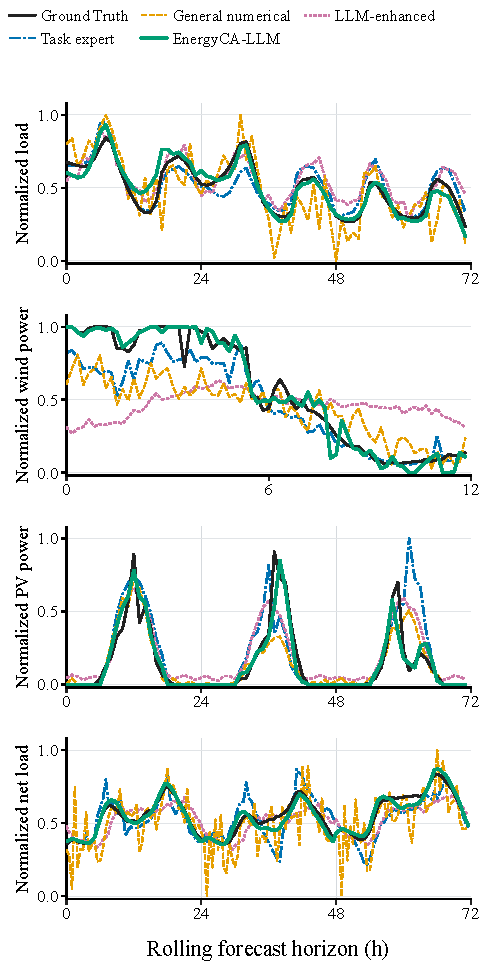
\includegraphics[width=\linewidth,trim=0bp 318bp 0bp 38.6128bp,clip]{Figures/fig_rolling_forecast_comparison.pdf}\par
{\footnotesize (a) Load}
\end{minipage}\hfill
\begin{minipage}[t]{0.48\textwidth}
\centering
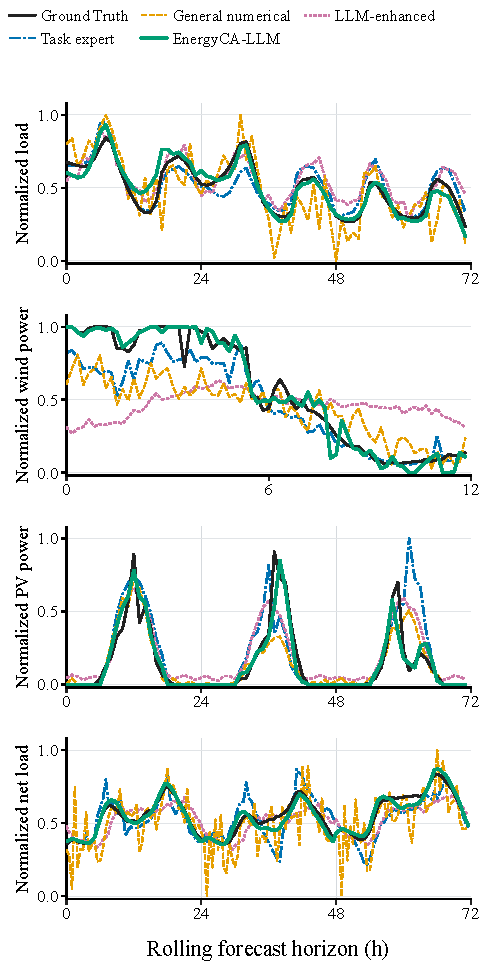
\includegraphics[width=\linewidth,trim=0bp 216bp 0bp 140.6128bp,clip]{Figures/fig_rolling_forecast_comparison.pdf}\par
{\footnotesize (b) Wind}
\end{minipage}\par
\vspace{6pt}
\begin{minipage}[t]{0.48\textwidth}
\centering
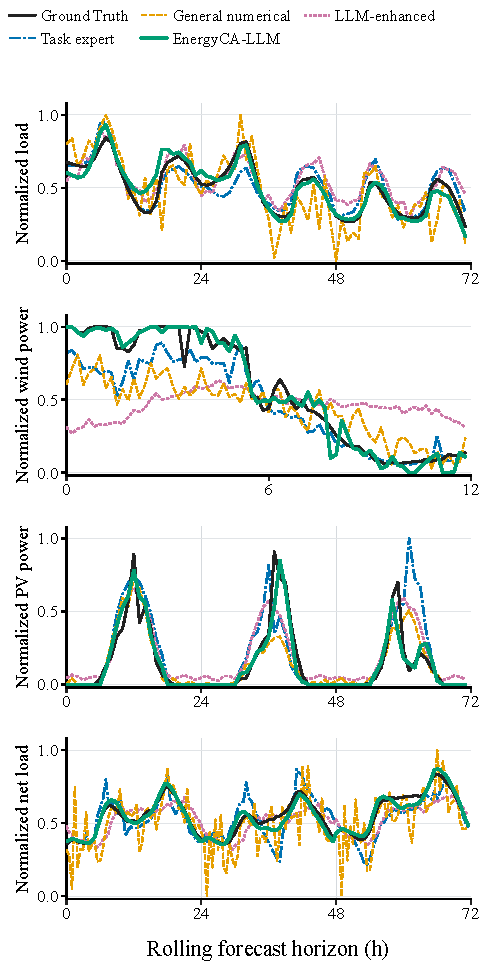
\includegraphics[width=\linewidth,trim=0bp 114bp 0bp 242.6128bp,clip]{Figures/fig_rolling_forecast_comparison.pdf}\par
{\footnotesize (c) PV}
\end{minipage}\hfill
\begin{minipage}[t]{0.48\textwidth}
\centering
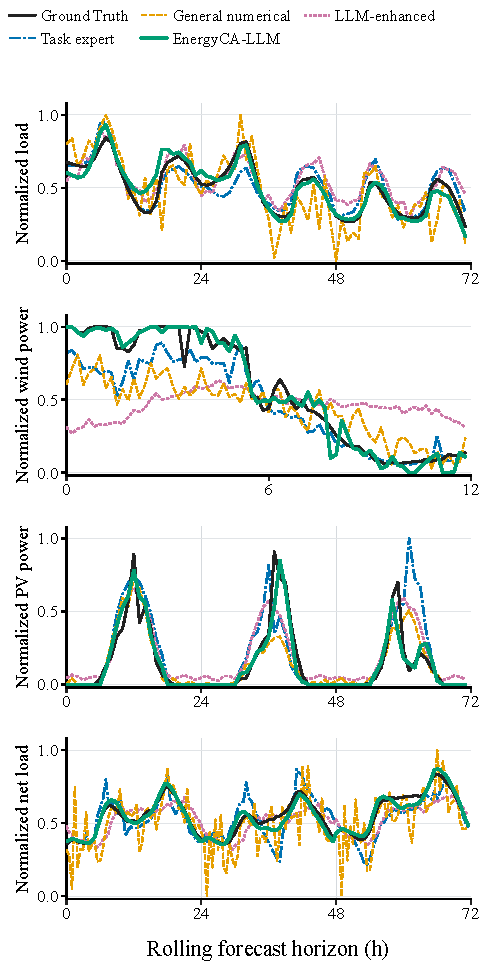
\includegraphics[width=\linewidth,trim=0bp 12bp 0bp 344.6128bp,clip]{Figures/fig_rolling_forecast_comparison.pdf}\par
{\footnotesize (d) Net load}
\end{minipage}\par
\vspace{3pt}
{\footnotesize Rolling forecast horizon (h)}
\caption{Illustrative normalized trajectories from the contextual-reference study: 12 hours for Wind and 72 hours for Load, PV and Net load. Each panel compares observations with representative general numerical, LLM-enhanced, task-expert and contextual-reference forecasts.}
\label{fig:task_specific_rolling_comparison}
\end{figure*}

\subsection{Cross-Task Reference Comparisons}

Table~\ref{tab:main_cross_task_results} compares NMAE, RMSE, sMAPE and daily seasonal MASE across Load, Wind, PV and Net load, while Figure~\ref{fig:task_specific_rolling_comparison} illustrates contextual-reference trajectories. Among the available Load comparisons, including joint-training results and the task-specific LSTM, Proposed has the lowest reported mean on all four metrics. It also leads all Wind metrics, PV NMAE/sMAPE/MASE and all Net-load metrics, with a four-task average validation MASE of $0.6967$; DLinear leads PV RMSE.








\subsection{Mechanism Ablations and Availability Robustness}
\label{sec:mechanism_ablation}

Table~\ref{tab:mechanism_ablation} separates four questions: the contribution of pretrained semantic representations (Panel A), joint semantic--numerical state construction (Panel B), shared low-rank bases and window-specific coefficients (Panel C), and explicit availability handling under incomplete or delayed context (Panel D). All four task columns report validation NMAE.

\begin{table*}[!tp]
\caption{Mechanism ablations of EnergyCA-LLM. Lower validation NMAE is better.}
\label{tab:mechanism_ablation}
\centering\footnotesize
\setlength{\tabcolsep}{0pt}
\renewcommand{\arraystretch}{1.08}
\newcolumntype{C}[1]{>{\centering\arraybackslash}p{#1}}
\begin{tabular}{@{}L{.32\textwidth}*{2}{C{.12\textwidth}}*{4}{C{.11\textwidth}}@{}}
\toprule
\multicolumn{7}{@{}l}{\textit{Panel A: Semantic representations}}\\
\midrule
Configuration & Pretrained & Frozen & Load & Wind & PV & Net load\\
\midrule
MLP schema encoder & No & No & 0.097716 & 0.718012 & \textbf{0.512839} & 0.081789\\
Frozen random Qwen3-8B & No & Yes & 0.095186 & \textbf{0.700191} & 0.525822 & 0.083679\\
\textbf{EnergyCA-LLM} & Yes & Yes & \textbf{0.090893} & 0.736146 & 0.513440 & \textbf{0.081151}\\
\bottomrule
\end{tabular}\par
\vspace{3pt}

\begin{tabular}{@{}L{.29\textwidth}*{3}{C{.09\textwidth}}*{4}{C{.11\textwidth}}@{}}
\toprule
\multicolumn{8}{@{}l}{\textit{Panel B: Joint window state and semantic--numerical interaction}}\\
\midrule
Configuration & Semantic & Numerical & Interaction & Load & Wind & PV & Net load\\
\midrule
Numerical-state control & No & Yes & No & 0.093102 & 0.718754 & \textbf{0.499328} & \textbf{0.081142}\\
Semantic-state control & Yes & No & No & 0.103931 & 0.714864 & 0.517679 & 0.091793\\
Concatenation only & Yes & Yes & No & 0.093661 & \textbf{0.681816} & 0.508760 & 0.087621\\
\textbf{EnergyCA-LLM} & Yes & Yes & Yes & \textbf{0.090893} & 0.736146 & 0.513440 & 0.081151\\
\bottomrule
\end{tabular}\par
\vspace{3pt}

\begin{tabular}{@{}L{.27\textwidth}C{.08\textwidth}C{.09\textwidth}C{.12\textwidth}*{4}{C{.11\textwidth}}@{}}
\toprule
\multicolumn{8}{@{}l}{\textit{Panel C: Residual bases and window-specific coefficients}}\\
\midrule
Configuration & Bases & Rank gate & Strength gate & Load & Wind & PV & Net load\\
\midrule
No residual adapter & -- & -- & -- & 0.103753 & 0.711702 & \textbf{0.501471} & 0.090916\\
Fixed shared adapter & Shared & Fixed & Fixed & 0.109850 & 0.758810 & 0.514037 & 0.090675\\
Task-specific bases & Per-task & Dynamic & Dynamic & 0.092101 & 0.740756 & 0.501597 & 0.088653\\
Rank gate only & Shared & Dynamic & Fixed & 0.097995 & 0.728389 & 0.509758 & 0.086319\\
Strength gate only & Shared & Fixed & Dynamic & 0.103456 & \textbf{0.701320} & 0.545252 & 0.088499\\
\textbf{EnergyCA-LLM} & Shared & Dynamic & Dynamic & \textbf{0.090893} & 0.736146 & 0.513440 & \textbf{0.081151}\\
\bottomrule
\end{tabular}\par
\vspace{3pt}

\begin{tabular}{@{}L{.34\textwidth}L{.22\textwidth}*{4}{C{.11\textwidth}}@{}}
\toprule
\multicolumn{6}{@{}l}{\textit{Panel D: Context-group availability robustness}}\\
\midrule
Configuration & Evaluation condition & Load & Wind & PV & Net load\\
\midrule
\multirow{3}{*}{\textbf{EnergyCA-LLM}} & Complete context & \textbf{0.090893} & 0.736146 & \textbf{0.513440} & \textbf{0.081151}\\
 & Group removal & \textbf{0.186066} & 0.803289 & \textbf{0.513440} & \textbf{0.081151}\\
 & 24-h delay & 0.137320 & \textbf{0.770504} & \textbf{0.513440} & \textbf{0.081151}\\
\midrule
\multirow{3}{*}{w/o group-availability encoding} & Complete context & 0.093171 & \textbf{0.709768} & 0.526940 & 0.084225\\
 & Group removal & 0.189205 & \textbf{0.764184} & 0.526940 & 0.084225\\
 & 24-h delay & \textbf{0.116935} & 1.081536 & 0.526940 & 0.084225\\
\bottomrule
\end{tabular}\par
\end{table*}

Panel A compares representations of the same eligible descriptive facts. The random and pretrained Qwen encoders share architecture, tokenizer and pooling, with language weights frozen; the MLP learns a structured-fact encoding. Panel B removes the semantic or pooled numerical state from both controller branches, while retaining availability and the original numerical predictor inputs. Concatenation-only control removes the product branch in Equation~\eqref{eq:window-residual-code}.

Panel C retains the predictor and gate generators. The task-specific control assigns separate rank-8 basis pairs to each task: 32,768 basis parameters versus 8,192 for shared bases. Both gates remain dynamic in that comparison. Other controls remove the adapter and its penalty or fix the indicated gate to one; the component rank remains eight.

Panel D compares models trained and selected under complete context, then evaluates the same selected checkpoints under group removal or a 24-hour delay. Group removal masks historical non-target, non-calendar covariates; delay masks their most recent 24 physical hours. Descriptors and availability are reconstructed at the corresponding observation cutoff while retaining target history and calendar inputs. The no-availability control omits explicit group-status text and zeros group-availability inputs to both the controller and known-future projection, retaining field-level masks. No perturbed validation score changes checkpoint selection.

All fits use seed 2027, the same data partitions and numerical preprocessing, and native $(L,H)$ interfaces $(168,24)$, $(1008,144)$, $(168,24)$ and $(336,52)$ for Load, Wind, PV and Net load. The pretrained variants share one frozen Qwen3-8B cache under each input condition. Each update accumulates equally weighted task losses at batch sizes $16,2,16,16$, clips the combined gradient at $1.0$ and applies AdamW with learning rate $3\times10^{-4}$, weight decay $10^{-4}$ and BF16 computation for 2,560 updates. Complete-context four-task mean validation asset-macro NMAE, evaluated every 128 updates, selects one shared checkpoint, with the earliest checkpoint retained on ties.

\section{Field-Level Language Representation Studies}
\label{sec:language_studies}

\subsection{Field Representation and Evaluation}

The field-conditioning reference uses Qwen3-8B representations of variable identity, physical unit and source role to condition target-guided historical-field attention and target queries, alongside scalar tokens formed from numerical values and masks. Unseen variable identifiers receive zero identity embeddings while retaining role, unit and description features. Physical-hour features encode historical offsets and forecast leads, and a seasonal anchor plus learned residual produces the output.

Evaluation covers one GEFCom2014 load zone, eight SDWPF turbines, eight MMSP/FusionSF PV sites and eight GSP regions, using the native interfaces in Section~\ref{sec:original_experiments}. Net load has 52 half-hour outputs at leads of 22--47.5 hours; Wind includes historical SCADA, and PV uses production histories. Within each comparison, partitions, fields, transformations and sample order are fixed. For asset $a$ in task $q$, let $A_{q,a}$ be mean absolute error over valid forecast targets and $S_{q,a}$ the training-set daily seasonal naive error. The asset-macro score and four-task mean are


\begin{equation}
\label{eq:language_study_mase}
\operatorname{MASE}_q=\frac{1}{|\mathcal A_q|}\sum_{a\in\mathcal A_q}\frac{A_{q,a}}{S_{q,a}},
\quad
\overline{\operatorname{MASE}}=\frac14\sum_{q\in\mathcal Q}\operatorname{MASE}_q.
\end{equation}
Daily periods are 24, 144, 24 and 48 steps for Load, Wind, PV and Net load~\cite{hyndman2006accuracy}. The field-level studies use seed 42 and select checkpoints by minimum four-task validation MASE, resolving equal scores by the earlier update.

\subsection{Paired Numerical and Language Adaptation}

The numerical, frozen-language and joint-language routes start from the same complete numerical checkpoint and receive 2,560 further updates with dropout disabled. The numerical route updates the final forecasting feed-forward block; frozen-language conditioning additionally learns a projection of fixed pretrained field vectors, and joint adaptation also updates Qwen LoRA parameters. The numerical block and semantic projection use peak learning rates $10^{-5}$ and $10^{-4}$, a 64-update warmup and cosine decay to 20\% of the peak. LoRA starts at update 129 with peak rate $3\times10^{-6}$ and its own 64-update warmup. Validation at update zero and every 128 updates selects update 2,432 for all three routes.

Frozen language conditioning reduces four-task mean validation MASE by 0.520\% relative to numerical adaptation, with joint adaptation adding a further 0.090\% reduction for a total of 0.610\%. Both language routes lower Load and Wind errors but increase PV and Net-load errors relative to the numerical route. Joint adaptation, in turn, lowers PV and Net-load errors relative to frozen conditioning while slightly increasing Load and Wind errors, so the aggregate gain combines different task responses to representation and optimization.

A complementary context-only comparison removes the direct structured-fact projection and runs 2,560 additional updates. Mean MASE is 0.702633 for a schema MLP, 0.750328 for frozen pretrained Qwen and 0.737411 for frozen random Qwen, versus 0.697762 for the numerical reference; the pretrained route selects update zero. The schema MLP leads the context-only routes, while the numerical reference has the lowest overall error in this comparison.

\subsection{SMARD Germany Cross-Dataset Zero-Shot Forecasting}
\label{sec:smard_zero_shot}

We evaluate frozen source-trained models on Germany DE grid load, total wind generation, photovoltaics and publisher residual load from SMARD. Target-domain data are used only for inference and scoring; checkpoints are selected using source validation. All comparisons use the same 358 coverage-valid daily forecast windows in 2024. The native task interfaces retain 24 hourly outputs for Load and PV, 144 ten-minute outputs for Wind, and 52 half-hour outputs at leads of 22--47.5 hours for Net load.

Inputs use visible same-task target history and the Europe/Berlin calendar, with unavailable source covariates masked. Visible-history median and scale provide per-window normalization. Hourly observations are causally held on subhourly grids, so these subhourly labels are proxies rather than independently observed measurements. The first seven days provide fixed daily seasonal scales for scoring. Table~\ref{tab:smard_zero_shot} reports three-seed mean MASE from unmodified forecasts; task-specific experts are evaluated only on their corresponding target. The Mean column averages the four task scores within each seed before aggregating across seeds. The existing Proposed transfer runs use the source-selected Qwen3-0.6B checkpoints over seeds 42, 2027 and 3407.

\begin{table}[!t]
\caption{SMARD Germany cross-dataset zero-shot test MASE.}
\label{tab:smard_zero_shot}
\centering\footnotesize
\setlength{\tabcolsep}{2pt}
\renewcommand{\arraystretch}{1.10}
\begin{tabular*}{\columnwidth}{@{\extracolsep{\fill}}lccccc@{}}
\toprule
Method & Load & Wind & PV & Net load & Mean \\
\midrule
DLinear & $\boldsymbol{1.027}$ & $0.746$ & $5.522$ & $1.106$ & $2.100$ \\
PatchTST & $1.242$ & $0.854$ & $11.522$ & $1.193$ & $3.703$ \\
TimeXer & $1.164$ & $0.838$ & $11.693$ & $1.294$ & $3.747$ \\
P2D-former & $1.114$ & $0.865$ & $14.431$ & $1.180$ & $4.397$ \\
DAMixer & $2.134$ & $0.971$ & $14.845$ & $1.405$ & $4.839$ \\
TFDNet & $1.114$ & $0.790$ & $10.292$ & $1.086$ & $3.320$ \\
Time-LLM & $1.079$ & $0.821$ & $11.559$ & $1.116$ & $3.644$ \\
CALF & $1.067$ & $0.828$ & $21.699$ & $1.319$ & $6.228$ \\
Load-GAM & $1.827$ & -- & -- & -- & -- \\
Load-LSTM & $1.437$ & -- & -- & -- & -- \\
KDD-GRU (adapted) & -- & $0.837$ & -- & -- & -- \\
2DXformer & -- & $0.961$ & -- & -- & -- \\
PV-GRU (adapted) & -- & -- & $16.996$ & -- & -- \\
Cross-Unet (adapted) & -- & -- & $16.573$ & -- & -- \\
Multiperiodic (adapted) & -- & -- & -- & $1.146$ & -- \\
Net-MLPFQR (adapted) & -- & -- & -- & $1.354$ & -- \\
\midrule
\textbf{Proposed} & $1.093$ & $\boldsymbol{0.734}$ & $\boldsymbol{4.619}$ & $\boldsymbol{1.056}$ & $\boldsymbol{1.875}$ \\
\bottomrule
\end{tabular*}
\end{table}

\subsection{CAISO Training-Label Budgets}
\label{sec:caiso_target_only}

The CAISO label-budget study uses a Qwen3-0.6B field-conditioning reference to load, wind, solar (including solar thermal) and official net demand. Forecasts issued at 00:00 Pacific time use 168 hourly observations with a two-hour buffer to predict 24 hours, with physical-hour queries determined by UTC offsets and calendar features in local time. Each field is centered by its visible-history median and scaled by the maximum of its historical interquartile range, $0.1$ times its mean absolute historical value and $10^{-8}$; the target field's offset and scale restore forecasts in MW.

Five randomly initialized numerical backbones use numerical prediction, a same-field MLP, frozen pretrained Qwen3-0.6B, frozen random Qwen3-0.6B or pretrained Qwen with LoRA. Training labels cover the earliest 7, 30 or 90 days from January 1, 2023; validation spans April 15--May 14, 2023, and the 2024 test set contains 354 valid daily forecast windows. Each fit uses seed 42 and 512 updates with selection including update zero. Daily seasonal scales are fixed from the earliest seven training days, and the reported score equally averages the four target MASE values.

\begin{table}[!t]
\caption{CAISO test performance by training-label budget, seed 42. Lower four-target mean MASE is better.}
\label{tab:caiso_target_only}
\centering\footnotesize
\setlength{\tabcolsep}{4pt}
\renewcommand{\arraystretch}{1.10}
\begin{tabular*}{\columnwidth}{@{\extracolsep{\fill}}lccc@{}}
\toprule
Configuration & 7 days & 30 days & 90 days \\
\midrule
Numerical model & 1.3606 & 1.2271 & 1.0476 \\
Same-field MLP & 1.3606 & 1.2841 & 1.0481 \\
Frozen pretrained Qwen & 1.3604 & \textbf{1.0258} & \textbf{0.9467} \\
Frozen random Qwen & \textbf{1.3378} & 1.2138 & 1.0496 \\
Pretrained Qwen + LoRA & 1.3604 & 1.0366 & 0.9481 \\
\bottomrule
\end{tabular*}
\end{table}

Frozen pretrained Qwen has the lowest four-target test MASE with 30 and 90 training days, reducing the numerical route's score by 16.40\% and 9.63\%, respectively; LoRA records 1.0366 and 0.9481 at these budgets. At seven days, the random encoder has the lowest score and all routes select their initial checkpoints. These supervised target-domain results, together with the context-only comparison, show that the benefit of pretrained conditioning varies with the numerical interface and training-label budget.



\Needspace{7\baselineskip}
\section{Conclusion}
\label{sec:conclusion}

EnergyCA-LLM combines frozen semantic encoding, numerical history and context-group availability to generate low-rank residual corrections after each temporal block of a shared Load, Wind, PV and Net-load predictor. Three-seed gate and availability studies characterize its task-specific responses to residual control and information conditions, complemented by reference studies of sharing and context encoders. In the field-conditioning study, paired language adaptation reduces four-task mean validation MASE by 0.610\% relative to numerical continuation, while frozen pretrained conditioning lowers CAISO four-target mean MASE by 16.40\% and 9.63\% with 30 and 90 training days. The shared-basis controller provides a common computation for zero-shot deployment by combining source-trained correction directions with coefficients generated from each target window.

\clearpage
\IEEEtriggeratref{22}
\bibliographystyle{IEEEtran}
\bibliography{references}
\end{document}
